\section{Circuit}

The circuit used for step three was inspired by the second simulated one from
step one.  With only one minor modification to the reference voltage, an
appropriate schematic is shown in Figure~\ref{f:schem}.
%
\begin{figure}[H]
\centering
	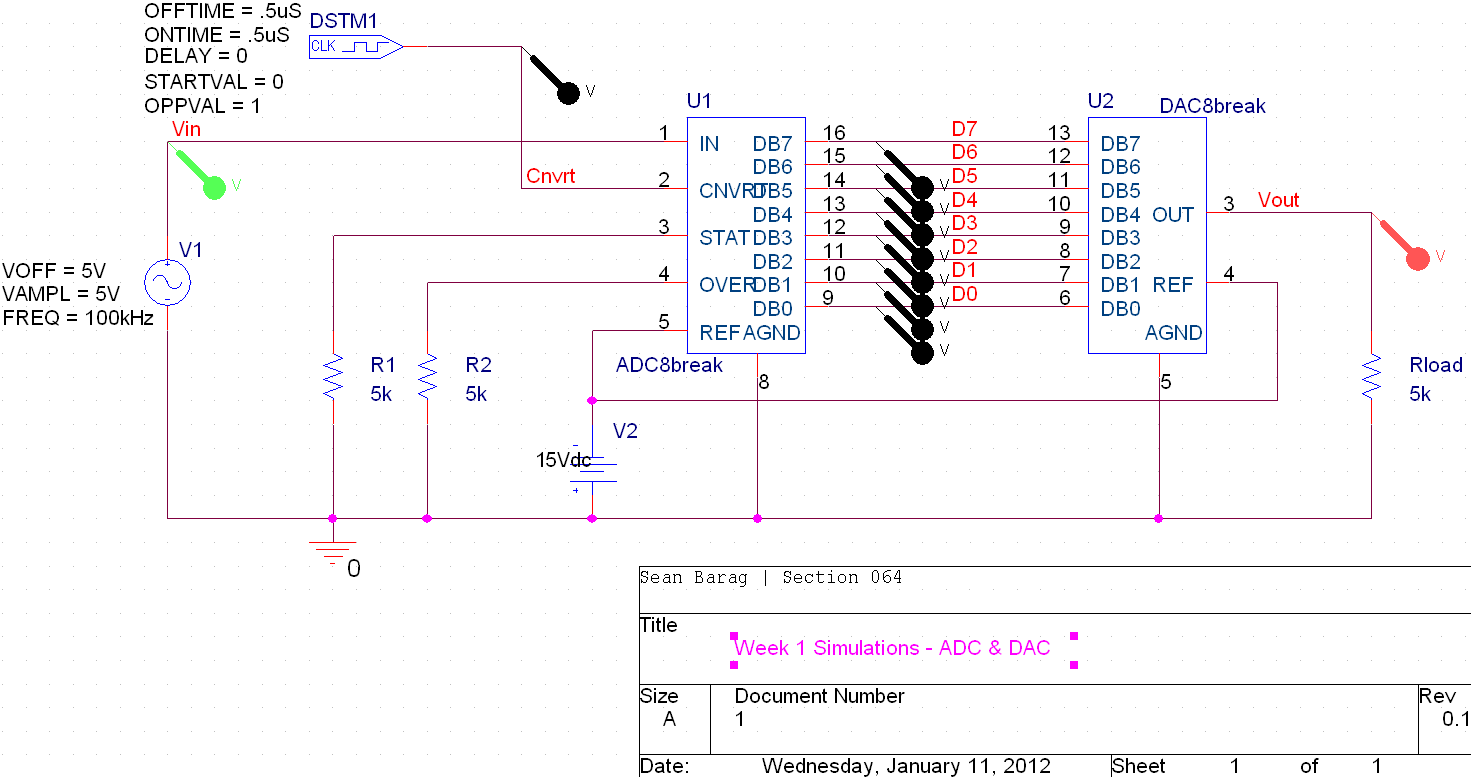
\includegraphics[width=.8\textwidth]{img/shot/schem.png}
	\parbox{.8\textwidth}{
	\caption[ADC-DAC Schematic]{Schematic for the ADC-DAC circuit being tested
	in step three.  It is logically similar to the one simulated in step one,
	but with a reference voltage of~\SI{-15}{\volt}.}
	\label{f:schem}}
\end{figure}
%
Because the circuit is so similar in design to the one originally described in
step one, a full explanation will be foregone here.  The only modifications to
take note of are a change in reference voltage~$V_\text{ref}$
to~\SI{-15}{\volt} and an input of varying frequency.
